\documentclass[fleqn]{NotesClass}

\usepackage{siunitx}
\usepackage{csquotes}
\usepackage{subcaption}
\usepackage{tikz-cd}

% Tikz stuff
\usepackage{tikz}
\tikzset{>=latex}
% external
\usetikzlibrary{external}
\tikzexternalize[prefix=tikz-external/]
%\tikzexternaldisable
% other libraries
\usetikzlibrary{hobby}
\usetikzlibrary{calc}
\usetikzlibrary{positioning}

% References, should be last things loaded
\usepackage{hyperref}  % Should be loaded second last (cleveref last)
\colorlet{hyperrefcolor}{blue!60!black}
\hypersetup{colorlinks=true, linkcolor=hyperrefcolor, urlcolor=hyperrefcolor}
\usepackage[
capitalize,
nameinlink,
noabbrev
]{cleveref} % Should be loaded last

% My packages
\usepackage{mathtools}
\usepackage{NotesBoxes}
\usepackage{NotesMaths}

% Title page info
\title{Statistical Physics}
\author{Willoughby Seago}
\date{}
% \subtitle{}
% \subsubtitle{}

% Highlight colour
\definecolor{highlight}{HTML}{00FF22}
\definecolor{my blue}{HTML}{00AAFF}
\definecolor{my red}{HTML}{FF2200}
\definecolor{my yellow}{HTML}{FFEE00}
\definecolor{my purple}{HTML}{CC00FF}

% Commands
% Maths
\newcommand*{\indicator}{\mathbf{1}}
\newcommand*{\order}{\mathcal{O}}
\newcommand*{\e}{\mathrm{e}}
\newcommand*{\boltzmann}{k_{\mathrm{B}}}

% Include
\includeonly{}

\begin{document}
    \frontmatter
    \titlepage
    \innertitlepage{tikz-external/the-ising-model.pdf}
    \tableofcontents
    \listoffigures
    \mainmatter
    
    \part{Monte Carlo and the Ising Model}
    \chapter{Monte Carlo}
    \defineindex{Monte Carlo} algorithms, named after the Monte Carlo casino, are stochastic methods for computing integrals.
    In a Monte Carlo computation we approximate the value of an integral by a series of averages.
    
    \section{Averages}
    Given a random variable, \(x_i\), the average is defined as
    \begin{equation}
        \expected{x} \coloneqq \frac{1}{n} \sum_{i=1}^{n} x_i
    \end{equation}
    where the sum is over all measurements of \(x\).
    Similarly if \(f\) is a function of the random variable \(x_i\) then the average value of this function is
    \begin{equation}
        \expected{f(x)} \coloneqq \frac{1}{n} \sum_{i=1}^{n} x_if(x_i) = \sum_{i=1}^{n} x_if_i
    \end{equation}
    where we define \(f_i = f(x_i)\).
    
    Often we instead want to work with weighted averages, say if certain outcomes are more likely than others.
    If outcome \(i\) has weight \(w_i\) then the weighted average of the random variable \(x_i\) is
    \begin{equation}
        \expected{x} \coloneqq \frac{\sum_{i=1}^{n} x_iw_i}{\sum_{i=1}^{n} w_i}.
    \end{equation}
    The weighted average of \(f\) is similarly
    \begin{equation}
        \expected{f(x)} \coloneqq \frac{\sum_{i=1}^{n} f(x_i)w_i}{\sum_{i=1}^{n}w_i}.
    \end{equation}
    
    \section{Monte Carlo Integration}
    Suppose we wish to compute the \(d\)-dimensional integral
    \begin{equation}
        I = \int_V f(\vv{r}) \dd{^dr}.
    \end{equation}
    First note that we can write this as an integral over all space by writing it as
    \begin{equation}
        I = \int_{\reals^d} f(\vv{r}) \indicator_V(\vv{r}) \dd{^dr}
    \end{equation}
    where \(\indicator_V\) is the indicator function for \(V\), defined by \(\indicator_V(\vv{r}) = 1\) if \(\vv{r} \in V\) and \(\indicator_V(\vv{r}) = 0\) if \(\vv{r} \notin V\).
    
    Using the fact that
    \begin{equation}
        V = \int_V \dl{^dr}
    \end{equation}
    is the volume of the integration region we can write the integral as
    \begin{equation}
        I = \frac{\int_V f(\vv{r}) \dl{^dr}}{\int_V \dl{^dr}} V.
    \end{equation}
    Notice now the similarity to the weighted average with all weights being 1, which is just the normal average, simply change integrals to sums.
    We therefore have
    \begin{equation}
        I = \frac{\int_V f(\vv{r}) \dd{^dr}}{\int_V \dl{^dr}} V \approx \frac{\sum_{i} f(\vv{r_i})}{\sum_i 1} = \expected{f(\vv{r})}.
    \end{equation}
    
    The process of calculating an integral becomes the process of computing an average.
    
    If we take \(n\) samples then the sum in the denominator is simply \(n\) and we have
    \begin{equation}
        I \approx \frac{\sum_{i=1}^{n} f_i}{n}V.
    \end{equation}
    This is our Monte Carlo estimate of the integral.
    
    The error on this measurement is associated with the standard error on the mean, since we are calculating a sample mean but really we want the population mean, that is \(n \to \infty\).
    The standard error on the mean is
    \begin{equation}
        \frac{\sigma}{\sqrt{n}} \sim n^{-1/2}
    \end{equation}
    where \(\sigma\) is the standard deviation.
    We clearly want \(n\) to be large in order to have a small error.
    
    \subsection{Trapezium Rule}
    An alternative method for approximating integrals is to split the integration region into sections, we then approximate \(f\) as linear over these sections.
    Define \(\overline{f_i}\) to be the average value of this linear approximation of \(f\) in the \(i\)th section.
    The integral is then approximated as the total volume of these sections that we have split the integral into.
    That is
    \begin{equation}
        I = \int_V f(\vv{r}) \dd{^d r} \approx \sum_i \text{volume of \(i\)th trapezium} = \sum_i \delta^d \overline{f_i}
    \end{equation}
    where \(\delta^d\) is the area of the base of the section, assuming we split the space evenly into a grid spaced \(\delta\) apart, and \(\overline{f_i}\) is the average height of the linear approximation of the function in this region.
    For a one-dimensional integral these small sections are trapeziums, hence the name trapezium rule.
    
    The error in our approximation of the function is \(\order(\delta^2)\) since we have approximated \(f\) as linear.
    The error then scales as \(n \delta^d \delta^2\) where \(n\) is the number of regions.
    The number of regions is the integration volume divided by the volume of each region, \(n = V/\delta^d\), and so \(\delta^d \sim 1/n\), which means \(\delta \sim n^{-1/d}\).
    The error therefore scales as \(nn^{-1}n^{-2/d} = n^{-2/d}\).
    
    Comparing this to the error for the Monte Carlo method we see that if \(d > 4\) the error on the Monte Carlo method actually decreases faster than the error for the more complex trapezium rule.
    
    \section{Statistical Physics}
    In statistical physics the Monte Carlo method can be used to compute thermodynamic averages.
    A system with a fixed number of particles, \(N\), is a canonical ensemble and the physics is dictated in part by the partition function
    \begin{equation}
        Z \coloneqq \sum_{\mathclap{i \in \{\text{states}\}}} \e^{-\beta E_i}
    \end{equation}
    where \(\beta \coloneqq 1/(\boltzmann T)\) with \(E_i\) being the energy of state \(i\), \(\boltzmann\) being Boltzmann's constant and \(T\) the temperature.
    
    The average of some observable, \(A\), is then given by summing over all states, \(i\):
    \begin{equation}
        \expected{A} \coloneqq \frac{\displaystyle\sum_{i} A_i\e^{-\beta E_i}}{\sum_{i} \e^{-\beta E_i}} = \frac{1}{Z} \sum_{i} A_i\e^{-\beta E_i}.
    \end{equation}
    That is \(\expected{A}\) is the weighted average with weight \(w_i = \e^{-\beta E_i}\).
    
    Writing this same value as
    \begin{equation}
        \expected{A} \approx \frac{\sum_{i=1}^{n} A_i\e^{-\beta E_i}}{n} \frac{n}{\sum_{i=1}^{n} \e^{-\beta E_i}},
    \end{equation}
    here we've introduced a factor of \(n/n = 1\), as well as approximating the sums over all states with sums over \(n\) states.
    Notice that the first term is the Monte Carlo estimate of the average of \(A\) and the second is the reciprocal of the Monte Carlo estimation of the partition function.
    
    The question is how we sample the states.
    The obvious answer of uniformly sampling the states turns out not to work, as we will see in the next section.
    
    \section{The Ising Model}
    The Ising model is a simple model that can be used to demonstrate several concepts in statistical mechanics.
    The \defineindex{Ising model} consists of a lattice of equally spaced points and we imagine that at each point there is a particle which can have either spin up or spin down.
    We will work with a two-dimensional grid.
    We index the points from \(1\) to \(N\), although we could also index each point by its row an column, which is often more useful in code.
    To each point \(i\) we assign a value of \(+1\) or \(-1\) depending on if the spin is up or down.
    We start with the spins chosen randomly and uniformly, so approximately half of the spins will be up and half down.
    
    \begin{figure}
        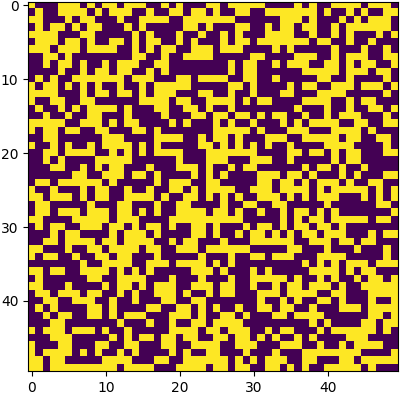
\includegraphics[height=0.3\textheight]{images/ising-random-start}
        \caption[Random Ising Model Start.]{Initially the Ising model starts in a random state. Here opposite spins are represented by different colours. The axes are simply the row and column numbers, here \(50^2 = 2500\) sites has been used.}
    \end{figure}
    
    The energy of the system depends only on how the spins align.
    We assume the grid spacing is large enough that only interactions with the nearest neighbours have effect.
    The total energy of the system is then
    \begin{equation}
        E = -J\sum_{\langle i, j \rangle} S_iS_j
    \end{equation}
    where \(J\) is a positive constant with dimensions of energy and \(\langle i, j \rangle\) means that we sum over \(i\) and then \(j\) corresponds to the nearest neighbours.
    
    \begin{figure}
        \tikzsetnextfilename{the-ising-model}
        \begin{tikzpicture}
            \fill[use Hobby shortcut, closed, highlight!20] (-0.5, 1) .. (0, 0.5) .. (0.4, 0.4) .. (0.5, 0) .. (1, -0.5) .. (1.5, 0) .. (1.6, 0.4) .. (2, 0.5) .. (2.5, 1) .. (2, 1.5) .. (1.6, 1.6) .. (1.5, 2) .. (1, 2.5) .. (0.5, 2) .. (0.4, 1.6) .. (0, 1.5);
            
            \draw[<-] (0, -0.25) -- ++ (0, 0.5);
            \draw[<-] (1, -0.25) -- ++ (0, 0.5);
            \draw[<-] (2, -0.25) -- ++ (0, 0.5);
            \draw[<-] (0, 0.75) -- ++ (0, 0.5);
            \draw[->] (1, 0.75) -- ++ (0, 0.5);
            \draw[->] (2, 0.75) -- ++ (0, 0.5);
            \draw[->] (0, 1.75) -- ++ (0, 0.5);
            \draw[<-] (1, 1.75) -- ++ (0, 0.5);
            \draw[->] (2, 1.75) -- ++ (0, 0.5);
            
            \node [left, font=\ttfamily\footnotesize] at (0, 2) {1};
            \node [left, font=\ttfamily\footnotesize] at (1, 2) {2};
            \node [left, font=\ttfamily\footnotesize] at (2, 2) {3};
            \node [left, font=\ttfamily\footnotesize] at (0, 1) {4};
            \node [left, font=\ttfamily\footnotesize] at (1, 1) {5};
            \node [left, font=\ttfamily\footnotesize] at (2, 1) {6};
            \node [left, font=\ttfamily\footnotesize] at (0, 0) {7};
            \node [left, font=\ttfamily\footnotesize] at (1, 0) {8};
            \node [left, font=\ttfamily\footnotesize] at (2, 0) {9};
        \end{tikzpicture}
        \caption[The Ising model.]{A \(3 \times 3\) Ising model with spins represented by arrows. The shaded region is the nearest neighbours of spin 5, the central spin.}
        \label{fig:ising model}
    \end{figure}

    \Cref{fig:ising model} shows a \(3\times 3\) Ising model.
    The nearest neighbours of the \(5\)th point are points 2, 4, 6, and 8.
    The contribution to the sum when \(i = 5\) is
    \begin{equation}
        -J\sum_{\langle 5, j \rangle} S_5S_j = -JS_5(S_2 + S_4 + S_6  + S_8) = -J 1(-1 - 1 + 1 - 1) = 2 J
    \end{equation}
    Notice that if we flip spin 5, that is \(S_5 \to -S_5\), the change in energy is
    \begin{align}
        \Delta E &= -J(-S_5)(S_2 + S_4 + S_6  + S_8) - (-J)S_5(S_2 + S_4 + S_6  + S_8)\\
        &= 2JS_5(S_2 + S_4 + S_6  + S_8)\\
        &= 2J1(-1 - 1 + 1 - 1)\\
        &= -4J
    \end{align}
    This can be used to avoid having to calculate the energy of the entire model when we flip a single spin.
    
    In a general Ising model of \(N\) sites, which in our example is 9, there are 2 possible values of the spin at each site and hence there are \(2^N\) possible states.
    In our example there are \(2^9 = 512\) possible states.
    A more realistic size would be a \(50 \times 50\) grid which has \(N = 50^2 = 2500\), in which case \(2^{2500} \approx = 10^{752}\), which is huge.
    
    The physics of the model is determined entirely by \(\e^{-\beta E}\).
    Since \(E \propto J\) the only values that appear in the model, apart from the values of the spins, is the product \(\beta J = J/(\boltzmann T)\).
    We could use real values for these, for example \(J\) would be some factor of \(\hbar\) and \(\boltzmann \approx 10^{-23}\,\unit{\joule\per\kelvin}\).
    However, these incredibly small numbers would cause huge floating point errors.
    Instead it is better to use the fact that these parameters only ever appear in ratio, \(J/\boltzmann\), and so we could just use \(J/\boltzmann \approx 10^{-12} \, \unit{\second \kelvin}\).
    This is still tiny however and will lead to floating point issues.
    A better thing to do is to set \(J = \boltzmann = 1\), and then use \(T\) as the parameter measured in some units such that \(J = \boltzmann = 1\).
    
    It is energetically favourable for all of the spins to align, either all up or all down.
    This means that there are two states which are much more likely than all other states, in particular they are much more likely than disordered states.
    On the other hand since \(2^N\) is likely very large the probability of getting either of these two states randomly is \(2^{-N}\), which is approximately zero.
    Instead we should generate states with weight \(\e^{-\beta E_i}\).
    This is called \defineindex{importance sampling}, where we generate states according to how likely they are, rather than uniform sampling.
    If we do this then we find that
    \begin{equation}
        \expected{A} = \frac{\sum_i A_i}{n},
    \end{equation}
    having already accounted for the factor of \(\e^{-\beta E_i}\) in our sampling.
    
    There are two ways to do this, which will be the topic of the next chapter.
    
    \chapter{Dynamics}
    \section{Markov Chains and the Metropolis Algorithm}
    As discussed in the previous chapter random uniform sampling is to simplistic for most physics simulations.
    Things don't happen in isolation, the surroundings have an important effect.
    Our goal in this chapter will be to develop a way of simulating this that allows us to select states in a way that reflects the underlying physics.
    We will do so using Markov chains and a version of the Metropolis algorithm.
    
    For our purposes a \defineindex{Markov chain} is a way of generating a new state based only on the current state in a way that is physically reasonable.
    If we start with the state \(\mu_1\), we can generate the state \(\mu_2\), and then from this we generate \(\mu_3\).
    Importantly the probability that \(\mu_3\) is a given state should depend only on \(\mu_2\), and not on \(\mu_1\).
    We say that the Markov chain is \enquote{memoryless} since it \enquote{can't remember \(\mu_1\)} once it leaves this state.
    
    After generating the states we will have a chain of states, \(\mu_1 \to \mu_2 \to \mu_3 \to \dotsb \to \mu_n\).
    The process for generating the next state is what we call the dynamics of the system.
    We will consider two different dynamical algorithms later in this chapter.
    
    The Metropolis algorithm is used in both dynamical algorithms which we will discuss.
    The general process for the metropolis algorithm is as follows.
    We start with the state \(\mu_i\) and we want to generate a state \(\mu_{i+1}\) in a physically reasonable way.
    \begin{cde}{Metropolis Algorithm}{}
        \begin{lstlisting}[gobble=12, escapechar=|]
            generate a new state, |\(\mu_{i + 1}\)|
            compute the energy change, |\(\Delta E\)|
            if |\(\Delta E < 0\)|:
                accept the new state, |\(\mu_{i + 1}\)|
            else:
                accept the new state with probability |\(\e^{-\beta \Delta E}\)|
            repeat until a new state has been accepted
        \end{lstlisting}
    \end{cde}
    An alternative way to state the if clause is to accept the new state with probability \(\min\{1, \e^{-\beta\Delta E}\}\).
    This algorithm is very simple, we just have to specify how to generate \(\mu_{i+1}\).
    
    \section{Glauber Dynamics}
    Glauber dynamics is the simplest algorithm for generating the next state.
    We simply choose a random site and flip the spin there.
    
    \subsection{Computing Energy}
    When deciding if we accept the result of this flip we need to compute \(\Delta E\).
    The naive way to do this is to calculate the total energy after the flip and before the flip and compute the difference.
    However, when doing this there is a lot of extra computation occurring that is unnecessary.
    Suppose that we choose to flip the \(i\)th spin for some fixed \(i\).
    Then
    \begin{equation}
        E_{\text{before}} = -J\sum_{\langle j, k \rangle} S_jS_k = -JS_i\sum_{\langle i, k \rangle} S_k - J\sum_{\substack{\langle j, k \rangle\\ j \ne i}} S_jS_k.
    \end{equation}
    Here \(S_i\) is the value \emph{before} the spin is flipped.
    Note that the sum over \(\langle i, k \rangle\) keeps \(i\) fixed and sums \(k\) over the nearest neighbours of \(i\).
    The energy after the spin is flipped is
    \begin{equation}
        E_{\text{before}} = J\sum_{\langle j, k \rangle} S_jS_k = -JS_i\sum_{\langle i, k \rangle} S_k - J\sum_{\substack{\langle j, k \rangle\\ j \ne i}} S_jS_k.
    \end{equation}
    Recall that the spins are represented by \(\pm 1\) so a spin flip is equivalent to a sign change.
    We can then compute the change in energy:
    \begin{equation}
        \Delta E = E_{\text{after}} - E_{\text{before}} = 2JS_i\sum_{\langle i, k \rangle} S_k.
    \end{equation}
    This is much quicker to compute and better yet can be done in constant time, \(\order(1)\).
    
    Sometimes we will need to compute the total energy of the system.
    The naive way to do this is to compute
    \begin{equation}
        E = -J\sum_{\langle i, j \rangle} S_iS_j
    \end{equation}
    where \(i\) now ranges over all sites and \(j\) takes on the value of the nearest neighbours indices.
    A better way to do this relies on recognising that each term in the sum is symmetric in \(i\) and \(j\).
    Therefore when computing, for example, the \(S_5S_6\) term we should also compute the \(S_6S_5\) term.
    For example, we may sum over the lattice but only account for the neighbours above and to the right, the neighbour to the left will be accounted for when we compute the term in the sum for the spin to the left and similarly with the site below.
    Both of these sums are \(\order(N)\) but by exploiting the symmetry like this the sum should be quicker to compute.
    
    \subsection{Results of Glauber Dynamics}
    The results with Glauber dynamics depend on the temperature.
    If the temperature is very high then \(\e^{-\beta\Delta E} \approx 1\) and so we always swap the spin, resulting in essentially random swaps and no order even after a long time.
    If the temperature is very low then \(\e^{-\beta\Delta E} \approx 0\) and we only swap the spin if the energy decreases.
    This means that we end up with alignment of spins increasing so we will eventually achieve a state where all of the spins are aligned.
    At low temperatures we can get stuck in a metastable state for a long time where we have two regions with opposite spins and the boundary contributes very little to the total energy and the chance of picking a state on the boundary is also low, resulting in a very slow change towards all the spins being aligned.
    
    \begin{figure}
        \begin{subfigure}[t]{0.45\textwidth}
            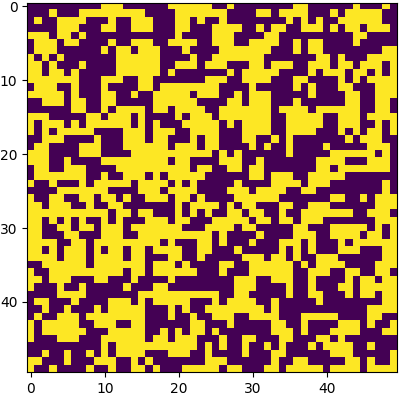
\includegraphics[width=0.95\textwidth]{images/ising-glauber-high-temp-result}
            \caption[The result of running Glauber dynamics at a high temperature.]{The result of running Glauber dynamics at a high temperature. Here a \enquote{high temperature} is \(T = 5\) in units where \(\boltzmann = J = 1\). Notice that the pattern of spins appears fairly random but there are slightly more yellow sites than purple.}
        \end{subfigure}
        \hspace{1em}
        \begin{subfigure}[t]{0.45\textwidth}
            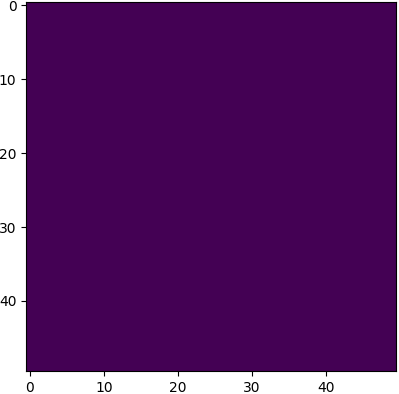
\includegraphics[width=0.95\textwidth]{images/ising-glauber-low-temp-result}
            \caption[The result of running Glauber dynamics at a low temperature.]{The result of running Glauber dynamics at a low temperature. Here a \enquote{low temperature} is \(T = 0.01\) in units where \(\boltzmann = J = 1\).}
        \end{subfigure}
        \begin{subfigure}[t]{0.45\textwidth}
            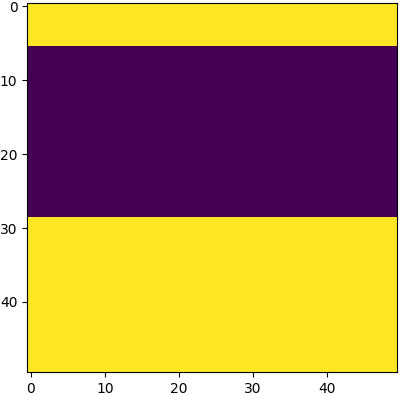
\includegraphics[width=0.95\textwidth]{images/ising-glauber-metastable}
            \caption[Metastable state]{A metastable state in the Glauber dynamics. The boundary being straight lines minimises the number of neighbouring unaligned spins. This state will remain for a long time but eventually all spins will align.}
        \end{subfigure}
        \hspace{1em}
        \begin{subfigure}[t]{0.45\textwidth}
            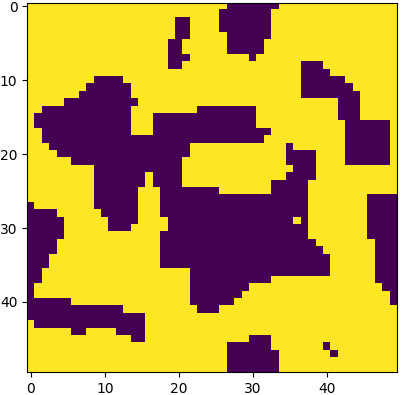
\includegraphics[width=0.95\textwidth]{images/ising-glauber-low-temp-part-way}
            \caption[A few steps into Glauber dynamics.]{The result of 10 sweeps with low temperature Glauber dynamics. One sweep meaning attempting to change \(N\) spins, where \(N\) is the total number of spins (here \(N = 2500\). Even after a relatively short time the spins separate into domains.}
        \end{subfigure}
        \caption{Various results of running Glauber dynamics for \(N = 50^2 = 2500\) spins.}
    \end{figure}
    
    \section{Kawasaki Dynamics}
    In Glauber dynamics we often end up with all spins aligned.
    This isn't always reasonable.
    Sometimes the net \defineindex{magnetisation} of a system,
    \begin{equation}
        M \coloneqq \sum_{i=1}^{N} S_i,
    \end{equation}
    is fixed.
    One way to model this sort of system is with Kawasaki dynamics.
    
    In Kawasaki dynamics we generate the next state by choosing two random spins and then swapping them.
    We now consider only what happens if the chosen spins are different since if their the same nothing changes.
    If these spins \emph{aren't} nearest neighbours then the change in energy is simply
    \begin{equation}
        \Delta E = 2JS_i \sum_{\langle i, k \rangle} S_k + 2JS_j \sum_{\langle j, l \rangle} S_l
    \end{equation}
    where \(i\) and \(j\) are the indices of the spins we swap.
    The logic for this is that this is essentially the same as repeating the Glauber dynamics process twice with these two spins chosen.
    
    If the spins are nearest neighbours then we have to be more careful calculating the energy change but it can still be done in an \(\order(1)\) way by carefully considering which spins are actually effected by the swap.
    
    Since we are only swapping spins the net magnetisation remains the same.
    This means that the results tend to have spins group into domains where they are all aligned since this minimises the energy.
    Of course if the temperature is high enough then entropy dominates and we get essentially random states indistinguishable from Glauber dynamics.
    
    % TODO: Add picture from Kawasaki dynamics
    
    \section{Measurements}
    Once we have a simulation running one of these dynamical algorithms we want to make measurements of the system.
    One of our goals will be to find the \defineindex{critical temperature}, \(T_{\mathrm{c}}\), which is the temperature at which the system goes from ordered to random.
    This is the temperature which distinguishes the \enquote{low temperature} cases from the \enquote{high temperature} cases.
    
    Two observables which we have already mentioned are the energy,
    \begin{equation}
        E = -J\sum_{\langle i, j \rangle} S_iS_j,
    \end{equation}
    and magnetisation,
    \begin{equation}
        M = \sum_{i=1}^{N} S_i.
    \end{equation}
    We expect that the energy will be much lower for an ordered phase and much higher for a disordered phase since spins align more in the ordered phase.
    For Glauber dynamics the magnetisation will tend to \(\pm N\) for low temperatures as all spins align.
    For this reason we consider the absolute value of the magnetisation, since there is nor real logic to assigning one spin as \(+1\) and the other as \(-1\) so the sign cannot have physical meaning.
    For Kawasaki dynamics \(M\) is constant so not that useful.
    
    The average energy is given by the Monte Carlo approximation as
    \begin{equation}
        \expected{E} = \frac{1}{n} \sum_{i=1}^{n} E(\mu_i)
    \end{equation}
    where \(\{\mu_i\}\) are all states visited and \(E(\mu_i)\) is the energy in state \(\mu_i\), and \(n\) is the total number of states visited, we take \(n\) to be large for this to be a good approximation.
    Similarly the average absolute magnetisation is
    \begin{equation}
        \expected{\abs{M}} = \frac{1}{n} \sum_{i=1}^{n} \abs{M(\mu_i)}
    \end{equation}
    where \(M(\mu_i)\) is the magnetisation in state \(\mu_i\).
    
    Consider what happens in Glauber dynamics.
    At a low temperature we expect that the spins align and so \(\expected{E} = -2JN\), since either \(S_i\) and \(S_j\) are both \(+1\) or both \(-1\), either way their product is \(+1\) and so we eventually achieve constant (up to random fluctuations of a few spins) energy \(-2JN\) and over enough time the states that occurred before achieving this have negligible impact on the average.
    At high temperatures the spins are essentially random so \(S_i\) and \(S_j\) are just as likely to have the same sign as the opposite sign and hence in the energy sum most terms cancel out and we get \(\expected{E} = 0\), again, up to random fluctuations.
    
    The case of magnetisation is similar with \(\expected{\abs{M}} = N\) at low temperatures and \(\expected{\abs{M}} = 0\) at high temperatures.
    
    % TODO: add images of plots showing results
    
    How can we use this to find the critical temperature?
    First we consider what happens when the number of spins, \(N\), tends to infinity.
    In this case we get two very clear regions of low and high temperature.
    This is shown in \cref{fig:averages for infinite spins}.
    Notice the discontinuity at the critical temperature, \(T_{\mathrm{c}}\).
    For small \(N\) however this discontinuity can't be seen.
    
    \begin{figure}
        \begin{tikzpicture}
            \draw[<->, very thick] (0, 4) node[above] {\(\expected{\abs{M}}\)} -- (0, 0) -- (4.2, 0) node[right] {\(T\)};
            \draw[ultra thick, highlight] (0, 3) -- ++ (2, 0) -- ++ (0, -3) -- ++ (2, 0);
            \node[below] at (2, 0) {\(T_{\mathrm{c}}\)};
            \begin{scope}[xshift=5cm]
                \draw[<-, very thick] (0, 4) node[above] {\(\expected{E}\)} -- (0, 0);
                \draw[->, very thick] (0, 3) -- (4.2, 3) node[right] {\(T\)};
                \draw[ultra thick, highlight] (0, 0.5) -- ++ (2, 0) -- ++ (0, 2.5) -- ++ (2, 0);
                \node[above] at (2, 3) {\(T_{\mathrm{c}}\)};
            \end{scope}
        \end{tikzpicture}
        \caption[Average absolute magnetisation and energy for an infinite number of spins.]{Plots of the average absolute magnetisation and energy for an infinite number of spins. Notice the sudden change at the critical temperature, \(T_{\mathrm{c}}\).}
        \label{fig:averages for infinite spins}
    \end{figure}
    
    Instead of the discontinuity we use the fact that fluctuations tend to be very large near the critical temperature as the system moves back and forth between the two phases.
    One measure of the fluctuations is the standard deviation,
    \begin{equation}
        \sigma_E \coloneqq \expected{E^2} - \expected{E}^2.
    \end{equation}
    However, by dividing by \(N\boltzmann T^2\) we can associate this with the specific heat capacity, \(C\), per spin:
    \begin{equation}
        \frac{\expected{E^2} - \expected{E}^2}{N\boltzmann T^2} = \frac{C}{N}.
    \end{equation}
    Similarly for the magnetisation we can relate the standard deviation to the susceptibility, \(\chi\), per spin:
    \begin{equation}
        \frac{\expected{M^2} - \expected{M}^2}{N\boltzmann T} = \frac{\chi}{N}.
    \end{equation}
    
    Plotting these quantities will give a peak at \(T_{\mathrm{c}}\).
    The height of the peak will vary with \(\ln N\) whereas away from the peak the values will be approximately constant with respect to \(N\).
    
    \section{Errors}
    \subsection{Autocorrelation and Equilibration Times}
    In order to avoid dependence on the initial conditions we should wait for the system to equilibrate before taking measurements.
    The easiest way to do this is to set some predefined wait time before starting measurements, rather than trying to asses whether the system is in equilibrium.
    The required time can be decreased when we are doing multiple simulation runs with slightly varied parameters by starting from the final state of the previous run.
    If we do this then an equilibration time of 100 sweeps is good enough for our purposes.
    
    If we were to make a measurement every sweep then the results would be highly correlated between neighbouring measurements.
    Instead we should wait some time, \(\tau_{\mathrm{a}}\), known as the \defineindex{autocorrelation time}.
    This can be defined by
    \begin{equation}
        \frac{\chi(t - t')}{\chi(0)} = \exp\left[ \frac{t - t'}{\tau_{\mathrm{a}}} \right],
    \end{equation}
    where \(\chi\) is the generalised susceptibility which we are measuring.
    The autocorrelation time is greatest near the point at which we get a phase transition, so we can compute a value at this point and use it for all simulation runs.
    It can be shown that an autocorrelation time of 10 sweeps between measurements is good enough for our purposes.
    
    \subsection{Estimating Errors}
    The error on zeroth order quantities like \(\expected{E}\) or \(\expected{\abs{M}}\) is easily computed as the standard error on the mean, which is the standard deviation divided by the mean:
    \begin{equation}
        \delta E = \frac{\sigma_{E}}{\expected{E}} = \sqrt{\frac{\expected{E^2} - \expected{E}^2}{n}},
    \end{equation}
    where \(n\) is the number of measurements of \(E\) that we made.
    
    This doesn't work so well for first order quantities, like
    \begin{equation}
        c = \frac{C}{N} = \frac{\expected{E^2} - \expected{E}^2}{N\boltzmann T^2} = \frac{1}{N} \diffp{\expected{E}}{T}.
    \end{equation}
    In order to get a good approximation of the error we would have to run the simulation lots of times and get lots of values of \(\expected{E}\) and \(\expected{E^2}\) and then take averages of these.
    There are other methods better suited to this case using resampling.
    
    The \defineindex{Bootstrap algorithm} for estimating the error in \(c = C/N\) is as follows:
    \begin{itemize}
        \item Start with \(n\) uncorrelated\footnote{for correlated measurements we need a few extra things, but we assume uncorrelated measurements since we wait for longer than the autocorrelation time between measurements.} measurements, e.g.\@ for \(n = 5\) we have \(E_1, \dotsc, E_5\).
        \item Resample, choose \(n\) measurements randomly from the set of all measurements, with replacement, e.g.\@ we might choose \(\{E_3, E_5, E_2, E_5, E_3\}\).
        \item Use the resampled set to compute \(c_i = C/N\).
        \item Repeat \(k\) times to generate \(\{c_1, \dotsc, c_k\}\).
        \item Estimate the error on \(c\) as \(\sigma_c = \sqrt{\expected{c^2} - \expected{c}^2}\) with \(\expected{c} = \sum_{i = 1}^k c_i / k\), and similar for \(\expected{c^2}\).
    \end{itemize}
    In practice we will take \(k \approx 100\) as a reasonable number of repeats for the bootstrap algorithm.
    
    The \defineindex{jacknife algorithm} for estimating the error in \(c = C/N\) is as follows:
    \begin{itemize}
        \item Start with \(n\) uncorrelated measurements, e.g.\@ for \(n = 5\) we have \(E_1, \dotsc, E_5\).
        \item Remove the first measurement for resampling, e.g.\@ \(E_2, E_3, E_4, E_5\).
        \item Compute \(c_1 = C/N\) using the data from the last step.
        \item Put the first measurement back and remove the second measurement, e.g.\@ \(E_1, E_3, E_4, E_5\).
        \item Compute \(c_2 = C/N\) using the data from the last step.
        \item \raisebox{-0.5ex}{\(\vdots\)}
        \item Put the \((i - 1)\)th measurement back and remove the \(i\)th, e.g.\@ \(E_1, \dotsc, E_{i-1}, E_{i+1}, \dotsc, E_5\).
        \item Compute \(c_i = C/N\) using the data from the last step.
        \item \raisebox{-0.5ex}{\(\vdots\)}
        \item Put the \((n - 1)\)th measurement back and remove the \(n\)th, e.g.\@ \(E_1, E_2, E_3, E_4\).
        \item Compute \(c_n = C/N\) using the data from the last step.
        \item Estimate the error as \(\sigma_c = \sqrt{\sum_{i=1}^k (c_i - \expected{c})^2} = \sqrt{k(\expected{c^2 - \expected{c}^2})}\).
    \end{itemize}
    
    Both the bootstrap and jacknife algorithms are reasonable for computing errors on first order measurements.
    However, the bootstrap algorithm has complexity \(\order(k)\) and the jacknife \(\order(n)\), and we will typically have \(k = 100\) and \(n \sim 10^3\), so bootstrap tends to be faster.
    Note that if there is still some correlation between measurements then both of these methods will under estimate the errors.
    
    \chapter{Why Does This Work?}
    \section{General Argument}
    \begin{rmk}
        The notion of detailed balance, key to the following discussion, is covered in the statistical physics notes.
    \end{rmk}
    Suppose we have completed a Markov chain simulation with the metropolis algorithm.
    This gives a chain of states, \(\mu_i\).
    Consider some particular state, \(\mu\).
    The probability that the system is in state \(\mu\) at time \(t\) is \(p_\mu(t)\).
    We want to know how fast this changes.
    To do so we need to consider the flux of states into \(\mu\) from some other state \(\nu\), and the flux of states out from \(\mu\) into some other state \(\nu\), and then sum over all states \(\nu\).
    To do this we need the transition probability for transition from \(\nu\) to \(\mu\), \(P(\nu \to \mu)\).
    Putting this together we get
    \begin{equation}
        \diffp{}{t}p_{\mu}(t) = \sum_{\nu \ne \mu} p_\nu(t) P(\nu \to \mu) - \sum_{\nu \ne \mu} p_{\mu}(t)P(\mu \to \nu).
    \end{equation}
    The first term represents the flux of states into \(\mu\) and the second the flux of states out of \(\mu\).
    
    We want to find \(p_\mu\) in steady state, that is when \(\diffp{p_\mu(t)}/{t} = 0\).
    We expect that
    \begin{equation}
        p_\mu \propto \exp[-\beta E_\mu]
    \end{equation}
    in steady state where \(\beta = 1/(\boltzmann T)\).
    This is just the Boltzmann distribution for a canonical ensemble.
    
    We define \(P(\mu \to \mu) = 0\) to allow us to write the equation above as a sum over all states.
    This means that in steady state we have
    \begin{equation}
        \diffp{p_\mu}{t} = \sum_{\nu}[p_\nu P(\nu \to \mu) - p_\mu P(\mu \to \nu)] = 0.
    \end{equation}
    It is not easy to solve this in general, but one solution is to have each term individually vanish.
    This is called \defineindex{detailed balance}.
    That is we have
    \begin{equation}
        p_\nu P(\nu \to \mu) = p_\mu P(\mu \to \nu)
    \end{equation}
    for all states \(\mu\) and \(\nu\).
    Taking \(\nu \ne \mu\) this gives
    \begin{equation}
        \frac{p_\mu}{p_\nu} = \frac{P(\nu \to \mu)}{P(\mu \to \nu)}.
    \end{equation}
    
    Given our ansatz of a Boltzmann distribution in steady state we look for
    \begin{equation}
        \frac{p_\mu}{p_\nu} = \exp[-\beta(E_\mu - E_\nu)].
    \end{equation}
    In Glauber dynamics we have
    \begin{equation}
        P(\mu \to \nu) = g(\mu \to \nu)A(\mu \to \nu)
    \end{equation}'	where \(g\) is the attempt rate, that is how often we select states \(\mu\) and \(\nu\), and \(A(\mu \to \nu)\) is the acceptance rate, that is, when we have selected states \(\mu\) and \(\nu\) what is the probability that we swap them.
    Recall that in Glauber dynamics one step involves flipping a single randomly chosen spin, and so
    \begin{equation}
        g(\mu \to \nu) = 
        \begin{cases}
            1/N & \text{if }\mu \text{ and } \nu \text{ differ by a single spin},\\
            0 & \text{otherwise}.
        \end{cases}
    \end{equation}
    Notice importantly that this means \(g(\mu \to \nu) = g(\nu \to \mu)\), and so this factor cancels in the ratio.
    We therefore want to choose \(A(\mu \to \nu)\) to give the desired ratio.
    The easiest way to do this is to take
    \begin{equation}
        A(\mu \to \nu) = \min\{1, \exp[-\beta(E_\nu - E_\mu)]\}.
    \end{equation}
    We then have
    \begin{align}
        \frac{p_\mu}{p_\nu} &= \frac{A(\nu \to \mu)}{A(\mu \to \nu)}\\
        &= 
        \begin{cases}
            \frac{\exp[-\beta(E_\mu - E_\nu)]}{1} & E_\mu > E_\nu\\
            \frac{1}{\exp[-\beta(E_\nu - E_\mu)]} & E_\mu < E_\nu
        \end{cases}
        \\
        &= \exp[-\beta(E_\mu - E_\nu)],
    \end{align}
    which is the desired result.
    
    We can make a similar argument to justify Kawasaki dynamics.
    The important thing is that, after a sufficient amount of time, both algorithms will take the system into an equilibrium state by imposing detailed balance.
    We are then free to take measurements and it will be as if we were drawing from a Boltzmann distribution.
    
    \part{Cellular Automata}
    \chapter{The Game of Life}
    \section{Cellular Automata}
    Cellular automata consist of a grid and a list of update rules for the grid depending on its current condition.
    There are many types of cellular automata.
    For example, the Ising model as discussed in the previous section is a cellular automata which is stochastic, meaning there is an element of randomness, and sequential, meaning we update one site at a time.
    We will now discuss a different cellular automata called the game of life which is deterministic, meaning the result depends only on the initial condition, and parallel, meaning we update all sites at the same time.
    
    \section{The Game of Life}
    The \defineindex{game of life} is a very simple cellular automata.
    To every cell we assign one of two states, \texttt{alive} or \texttt{dead}.
    We then update all cells at once based on the following algorithm.
    \begin{itemize}
        \item An \texttt{alive} cell with fewer than 2 neighbours becomes a \texttt{dead} cell.
        \item An \texttt{alive} cell with more than 3 neighbours becomes a \texttt{dead} cell.
        \item A \texttt{dead} cell with exactly three \texttt{alive} neighbours becomes \texttt{alive}.
        \item An \texttt{alive} cell with 2 or 3 \texttt{alive} neighbours remains \texttt{alive}.
    \end{itemize}
    Note that in the game of live neighbours includes diagonals, so each cell has 8 neighbours.
    
    Despite the simple rules the game of life can develop very complex systems.
    
    \subsection{Final States}
    An \defineindex{absorbing state} is one in which the system stops changing.
    An ergodic system, one in which all possible states are visited, cannot have absorbing states, but the game of life is not ergodic so this is not of concern.
    One example of an absorbing state is the \texttt{block}.
    This consists of a \(2\times 2\) block of \texttt{alive} cells surrounded by \texttt{dead} cells.
    This is shown in \cref{fig:game of life block state}.
    Another slightly more complicated absorbing state is the \texttt{beehive}, shown in \cref{fig:game of life beehive state}.
    
    \begin{figure}
        \tikzsetnextfilename{game-of-life-block}
        \begin{tikzpicture}
            \foreach \x/\y in {1/1, 1/2, 2/1, 2/2} {
                \coordinate (A) at (\x, \y);
                \fill[my blue] (A) rectangle ($(A) + (1, 1)$);
            }
            \draw[thick] (0, 0) grid (4, 4);
            \begin{scope}[xshift=5cm]
                \foreach \x/\y in {1/1, 1/2, 2/1, 2/2} {
                    \coordinate (A) at (\x, \y);
                    \fill[my blue!50] (A) rectangle ($(A) + (1, 1)$);
                    \node at ($(A) + (0.5, 0.5)$) {3};
                }
                \foreach \x/\y in {0/0, 0/3, 3/3, 3/0} {
                    \node at ($(\x, \y) + (0.5, 0.5)$) {1};
                }
                \foreach \x/\y in {0/1, 0/2, 1/0, 2/0, 3/1, 3/2, 1/3, 2/3} {
                    \node at ($(\x, \y) + (0.5, 0.5)$) {2};
                }
                \draw[thick, black!50] (0, 0) grid (4, 4);
            \end{scope}
        \end{tikzpicture}
        \caption[Game of life \texttt{block} state.]{The \texttt{block} state is an absorbing state of the game of life. All \texttt{alive} cells have 3 neighbours and no dead cells have 3 neighbours, so noting changes.}
        \label{fig:game of life block state}
    \end{figure}

    \begin{figure}
        \tikzsetnextfilename{game-of-life-beehive}
        \begin{tikzpicture}
            \foreach \x/\y in {2/1, 1/2, 3/2, 1/3, 3/3, 2/4} {
                \coordinate (A) at (\x, \y);
                \fill[my blue] (A) rectangle ($(A) + (1, 1)$);
            }
            \draw[thick] (0, 0) grid (5, 6);
            
            \begin{scope}[xshift=6cm]
                \foreach \x/\y in {2/1, 1/2, 3/2, 1/3, 3/3, 2/4} {
                    \coordinate (A) at (\x, \y);
                    \fill[my blue!50] (A) rectangle ($(A) + (1, 1)$);
                }
                \foreach \x/\y in {0/0, 0/5, 4/0, 4/5} {
                    \node at ($(\x, \y) + (0.5, 0.5)$) {0};
                }
                \foreach \x/\y in {1/0, 2/0, 3/0, 1/5, 2/5, 3/5, 0/1, 0/4, 4/1, 4/4} {
                    \node at ($(\x, \y) + (0.5, 0.5)$) {1};
                }
                \foreach \x/\y in {1/1, 2/1, 3/1, 1/4, 2/4, 3/4, 0/2, 0/3, 1/2, 1/3, 3/2, 3/3, 4/2, 4/3} {
                    \node at ($(\x, \y) + (0.5, 0.5)$) {2};
                }
                \foreach \x/\y in {2/2, 2/3} {
                    \node at ($(\x, \y) + (0.5, 0.5)$) {5};
                }
                \draw[thick, black!50] (0, 0) grid (5, 6);
            \end{scope}
        \end{tikzpicture}
        \caption[Game of life \texttt{beehive} state.]{The \texttt{beehive} state is an absorbing state of the game of life. All \texttt{alive} cells have 2 neighbours and no dead cells have 3 neighbours, so nothing changes.}
        \label{fig:game of life beehive state}
    \end{figure}
    
    Another option is an oscillating state.
    These are states which change, but follow a fixed pattern which eventually repeats.
    The simplest oscillator is the \texttt{blinker}, which consists of a \(3\times 1\) block of \texttt{alive} states, which turns into a \(1 \times 3\) block of \texttt{alive} states, which turns back into the original \(3\times 1\) block of \texttt{alive} states.
    This is shown in \cref{fig:game of life blinker state}.
    
    \begin{figure}
        \tikzsetnextfilename{game-of-life-blinker}
        \begin{tikzpicture}
            \foreach \x/\y in {1/2, 2/2, 3/2} {
                \coordinate (A) at (\x, \y);
                \fill[my blue] (A) rectangle ($(A) + (1, 1)$);
            }
            \draw[thick] (0, 0) grid (5, 5);
            \draw[->, thick] (2, -0.5) to[bend right] (2, -1.5);
            \draw[->, thick] (3, -1.5) to[bend right] (3, -0.5);
            
            \begin{scope}[xshift=6cm]
                \foreach \x/\y in {1/2, 2/2, 3/2} {
                    \coordinate (A) at (\x, \y);
                    \fill[my blue!50] (A) rectangle ($(A) + (1, 1)$);
                }
                
                \foreach \x/\y in {0/0, 1/0, 2/0, 3/0, 4/0, 0/4, 1/4, 2/4, 3/4, 4/4} {
                    \node at ($(\x, \y) + (0.5, 0.5)$) {0};
                }
                \foreach \x/\y in {0/1, 0/2, 0/3, 4/1, 4/2, 4/3, 1/2, 3/2} {
                    \node at ($(\x, \y) + (0.5, 0.5)$) {1};
                }
                \foreach \x/\y in {1/1, 3/1, 1/3, 3/3, 2/2} {
                    \node at ($(\x, \y) + (0.5, 0.5)$) {2};
                }
                \foreach \x/\y in {2/1, 2/3} {
                    \node at ($(\x, \y) + (0.5, 0.5)$) {3};
                }
                \draw[thick, black!50] (0, 0) grid (5, 5);
                \draw[->, thick] (2, -0.5) to[bend right] (2, -1.5);
                \draw[->, thick] (3, -1.5) to[bend right] (3, -0.5);
            \end{scope}
            
            \begin{scope}[yshift=-7cm]
                \foreach \x/\y in {2/1, 2/2, 2/3} {
                    \coordinate (A) at (\x, \y);
                    \fill[my blue] (A) rectangle ($(A) + (1, 1)$);
                }
                \draw[thick] (0, 0) grid (5, 5);
            \end{scope}
            
            \begin{scope}[xshift=6cm, yshift=-7cm]
                \foreach \x/\y in {2/1, 2/2, 2/3} {
                    \coordinate (A) at (\x, \y);
                    \fill[my blue!50] (A) rectangle ($(A) + (1, 1)$);
                }
                
                \foreach \x/\y in {0/0, 0/1, 0/2, 0/3, 0/4, 4/0, 4/1, 4/2, 4/3, 4/4} {
                    \node at ($(\x, \y) + (0.5, 0.5)$) {0};
                }
                \foreach \x/\y in {1/0, 2/0, 3/0, 1/4, 2/4, 3/4, 2/1, 2/3} {
                    \node at ($(\x, \y) + (0.5, 0.5)$) {1};
                }
                \foreach \x/\y in {1/1, 1/3, 3/1, 3/3, 2/2} {
                    \node at ($(\x, \y) + (0.5, 0.5)$) {2};
                }
                \foreach \x/\y in {1/2, 3/2} {
                    \node at ($(\x, \y) + (0.5, 0.5)$) {3};
                }
                \draw[thick, black!50] (0, 0) grid (5, 5);
            \end{scope}
        \end{tikzpicture}
        \caption[Game of life \texttt{blinker} state.]{The \texttt{blinker} state is an oscillating state of the game of life. Two \texttt{alive} cells only have one \texttt{alive} neighbour, so become \texttt{dead} cells, and two \texttt{dead} cells have three \texttt{alive} neighbours and so become \texttt{alive}. The same then happens but rotated by \ang{90}. This state then returns to the original state.}
        \label{fig:game of life blinker state}
    \end{figure}
    
    The period of an oscillating state is how many states it visits before the pattern starts repeating.
    The blinker is a period 2 oscillator, since it has two states.
    Diagrammatically we can write a period two oscillator as
    \begin{equation}
        \tikzsetnextfilename{game-of-life-period-two-oscillator}
        \begin{tikzpicture}[baseline=(current bounding box)]
            \node (A) {\(A\)};
            \node[right=of A] (B) {\(B\).};
            \draw[->] (A) to[bend right] (B);
            \draw[->] (B) to[bend right] (A);
        \end{tikzpicture}
    \end{equation}
    A period three oscillator can the be represented as
    \begin{equation}
        \tikzsetnextfilename{game-of-life-period-three-oscillator}
        \begin{tikzpicture}[baseline=(current bounding box)]
            \node (A) {\(A\)};
            \node (B) at (-60:1) {\(B\).};
            \node (C) at (-120:1) {\(C\)};
            \draw[->] (A) to[bend left] (B);
            \draw[->] (B) to[bend left] (C);
            \draw[->] (C) to[bend left] (A);
        \end{tikzpicture}
    \end{equation}
    Notice that the existence of period three oscillators breaks time reversal symmetry since
    \begin{equation}
        \tikzsetnextfilename{game-of-life-period-three-oscillator-forwards}
        \begin{tikzpicture}[baseline=-4ex]
            \node (A) {\(A\)};
            \node (B) at (-60:1) {\(B\)};
            \node (C) at (-120:1) {\(C\)};
            \draw[->] (A) to[bend left] (B);
            \draw[->] (B) to[bend left] (C);
            \draw[->] (C) to[bend left] (A);
        \end{tikzpicture}
        \ne
        \tikzsetnextfilename{game-of-life-period-three-oscillator-backwards}
        \begin{tikzpicture}[baseline=-4ex]
            \node (A) {\(A\)};
            \node (B) at (-60:1) {\(B\).};
            \node (C) at (-120:1) {\(C\)};
            \draw[->] (A) to[bend right] (C);
            \draw[->] (C) to[bend right] (B);
            \draw[->] (B) to[bend right] (A);
        \end{tikzpicture}
    \end{equation}
    
    Another class of final states is travelling states.
    These are somewhat like oscillators, in that the same arrangement of \texttt{alive} cells occurs over and over, but the position of these cells changes.
    The simplest travelling state is the \texttt{glider}.
    This is shown in \cref{fig:game of life glider state}.
    The \texttt{glider} has period four, meaning that there are four distinct arrangements of cells, but as a travelling state the game doesn't return to exactly the same state, rather a translated version.
    
    \begin{figure}
        \tikzsetnextfilename{game-of-life-glider}
        \begin{tikzpicture}
            \foreach \x/\y in {1/1, 2/1, 3/1, 3/2, 2/3} {
                \coordinate (A) at (\x, \y);
                \fill[my blue] (A) rectangle ($(A) + (1, 1)$);
            }
            \draw[thick] (0, 0) grid (5, 5);
            
            \begin{scope}[xshift=6cm]
                \foreach \x/\y in {1/1, 2/1, 3/1, 3/2, 2/3} {
                    \coordinate (A) at (\x, \y);
                    \fill[my blue!50] (A) rectangle ($(A) + (1, 1)$);
                }
                
                \foreach \x/\y in {0/3, 0/4, 4/4} {
                    \node at ($(\x, \y) + (0.5, 0.5)$) {0};
                }
                \foreach \x/\y in {0/0, 4/0, 0/1, 0/2, 1/3, 4/3, 1/4, 2/4, 3/4, 1/1, 2/3} {
                    \node at ($(\x, \y) + (0.5, 0.5)$) {1};
                }
                \foreach \x/\y in {1/0, 3/0, 4/1, 4/2, 3/3, 3/1} {
                    \node at ($(\x, \y) + (0.5, 0.5)$) {2};
                }
                \foreach \x/\y in {2/0, 2/1, 1/2, 3/2} {
                    \node at ($(\x, \y) + (0.5, 0.5)$) {3};
                }
                \foreach \x/\y in {2/2} {
                    \node at ($(\x, \y) + (0.5, 0.5)$) {5};
                }
                \draw[thick, black!50] (0, 0) grid (5, 5);
            \end{scope}
        \end{tikzpicture}
        \caption[Game of life \texttt{glider state}]{The \texttt{glider} state is a travelling state of the game of life. The current configuration will move diagonally down and right.}
        \label{fig:game of life glider state}
    \end{figure}
    
    One question we may want to ask is how fast a travelling state is.
    To do this we calculate the centre of mass of the state.
    This can be done using
    \begin{equation}
        \vv{r_{\mathrm{cm}}} = \frac{1}{n} \sum_{i = 2}^n \vv{r_i}a_i ,
    \end{equation}
    where \(n\) is the number of cells, \(\vv{r_i}\) is the position of the \(i\)th cell, and \(a_i\) is 0 if cell \(i\) is \texttt{dead} and 1 if cell \(i\) is \texttt{alive}.
    We can then work out the velocity of the centre of mass by working out the displacement after \(t\) steps and then dividing by \(t\).
    
    Another sensible question is how long it takes a given scenario to reach a final state, by which we mean a state in which noting is really going to change, including states with non-interacting oscillators and travelling states.
    To do this we can simply count the number of alive cells over some period and if it doesn't change for a sufficiently large amount of time we say we've reached a final state.
    It is possible that a given initial state may not reach a final state by this definition, or may take a very long time, but most initial states that will result in a final state will do so in less than 5000 steps.
    
    \chapter{SIRS Model}
    \section{The SIRS Model}
    The \defineindex{SIRS model} is a basic stochastic sequential cellular automata for modelling epidemics.
    There are three states, \texttt{S}, \texttt{I}, and \texttt{R}.
    These stand for susceptible, infected, and recovered.
    Each step a site is picked and the following rules applied:
    \begin{itemize}
        \item If the site is in state \texttt{S} and it has at least one infected neighbour it will change to state \texttt{I} with probability \(p_1\).
        This represents the infected neighbour infecting the susceptible site.
        \item If the site is in state \texttt{I} it will change to state \texttt{R} with probability \(p_2\).
        This represents the infected site recovering from the illness.
        \item If the site is in state \texttt{R} it will change to state \texttt{S} with probability \(p_3\).
        This represents the recovered site losing immunity.
    \end{itemize}
    Note that in the SIRS model we take only the cells to the left, right, above, and below as neighbours, not the diagonals.
    
    It should be noted that the SIRS model is a slight modification of the SIR model, which doesn't allow for recovered states becoming susceptible again, essentially states in the SIR model have permanent immunity after recovering.
    
    Note that once a rule has been applied we finish the step, otherwise it would be possible to have a single site go from \texttt{S} to \texttt{I} to \texttt{R} and back to \texttt{S} in one step.
    
    \section{Phases}
    There are three phases, which we characterise with the order parameter \(I/N\), where \(I\) is the number of sites in state \texttt{I} and \(N\) is the number of steps completed.
    The first state is the absorbing state, where \(I/N\) eventually becomes 0.
    This represents no infected people, so only susceptible and recovered people.
    Eventually this will become only susceptible people, but this last bit isn't of interest, and we stop once the illness vanishes.
    
    The second state is dynamic equilibrium.
    In this \(I/N\) is approximately constant with only small fluctuations.
    This represents something like a mild flu.
    
    The final state is somewhere between these two states and is a wave state.
    In this \(I/N\) fluctuates between almost zero and most people being infected.
    We can identify this by considering the variance, \((\expected{I^2} - \expected{I}^2) / N\), which will be large for a wave phase.
    
    We can study these different phases by fixing \(p_3\), for example, and then considering a range of values for \(p_1\) and \(p_2\) and producing a heat map of \(\expected{I}/N\).
    We can also fix, for example, \(p_2\), and consider just a range of values of \(p_1\) if we want higher resolution measurements.
    
    \section{Immunity}
    One modification we can make is to introduce a fourth state, \texttt{Im}, representing permanent immunity, say a genetic immunity that only some people have.
    Sites in this state cannot become another state, and likewise sites that don't start in this state cannot move into this state.
    We can then study the behaviour of \(\expected{I}/N\) as a function of \(f_{\mathtt{Im}}\), which is the fraction of people who start in state \texttt{Im}.
    We expect that \(\expected{I}/N\) decreases as \(f_{\mathrm{Im}}\) increases.
    At some point \(\expected{I}/N\) will be zero for sufficiently large \(f_{\mathtt{Im}}\).
    This represents herd immunity.
    
    \part{Partial Differential Equations}
    \chapter{Initial Value Problems}
    \section{Types of PDEs}
    Broadly there are two types of partial differential equations (PDEs).
    These are initial value problems (IVPs) in which we have some system evolving in time and we know its state at time \(t = 0\), and boundary value problems (BVPs) in which we have some system evolving in space and we know its value on a boundary.
    An example of an initial value problem is the diffusion equation,
    \begin{equation}
        \diffp{c}{t} = D\laplacian c,
    \end{equation}
    where \(c(\vv{r}, t)\) is the concentration of some quantity at position \(\vv{r}\) and time \(t\) and \(D\) is a constant.
    In order to solve this we need to know \(c(\vv{r}, 0)\) for all \(\vv{r}\).
    An example of a boundary value problem is Poisson's equation,
    \begin{equation}
        \laplacian\varphi = -\frac{\rho}{\varepsilon},
    \end{equation}
    where \(\varphi(\vv{r})\) is the electric potential due to some fixed charge density, \(\rho(\vv{r})\).
    In order to solve a boundary value problem we need to know boundary conditions.
    These come in two forms.
    \defineindex{Dirichlet boundary conditions} involve knowing the value of \(\varphi\) along some boundary, and \defineindex{von Neumann boundary conditions} involve knowing the value of \(\vh{n}\cdot\grad\varphi\) along some boundary where \(\vh{n}\) is a unit vector normal to the boundary.
    
    In this chapter we are interested in initial value problems, which are typically easier to solve.
    
    \section{IVP: Diffusion in One Dimension}
    Consider the one-dimensional diffusion equation
    \begin{equation}
        \diffp{c}{t} = D\diffp[2]{c}{x},
    \end{equation}
    where \(c(x, t)\) is the concentration.
    We will solve this with a \defineindex{finite difference} method, which entails approximating derivatives, defined by the limit
    \begin{equation}
        \diffp{c}{t} \coloneqq \lim_{\delta t \to 0} \frac{c(x, t + \delta t) - c(x, t)}{\delta t}.
    \end{equation}
    by replacing \(\delta t\) with some small but non-zero value.
    To do so we discretise space into points separated by a distance \(\delta x\).
    We then label these points by \(i\).
    We also discretise time into steps of size \(\delta t\), so that \(t = n \delta t\), and we can use \(n\) to label times.
    We can then approximate the derivative at \(x = i\delta x\) and time \(t = n\delta t\) by
    \begin{equation}
        \diffp{c}{t} \approx \frac{c[i; n + 1] - c[i; n]}{\delta t}.
    \end{equation}
    This is called the \defineindex{forward difference} approximation, since it involves using the current time, \(n\), and the next time, \(n + 1\).
    We can also compute the \defineindex{backward difference} approximation:
    \begin{equation}
        \diffp{c}{t} \approx \frac{c[i; n] - c[i; n - 1]}{\delta t}.
    \end{equation}
    These should give similar results for sufficiently small values of \(\delta t\), and it is only when computing higher order derivatives, where errors compound, that we have to be careful about which we use.
    
    Now consider \(c(x + \delta x, t)\).
    We can Taylor expand this quantity, giving
    \begin{equation}
        c(x + \delta x, t) \approx c(x, t) + \delta x\diffp{c}{x}[(x,t)] + \frac{\delta x^2}{2}\diffp[2]{c}{x}[(x,t)] + \order(\delta x^3).
    \end{equation}
    Similarly we have
    \begin{equation}
        c(x - \delta x, t) \approx c(x, t) - \delta x\diffp{c}{x}[(x, t)] + \frac{\delta x^2}{2}\diffp[2]{c}{x}[(x, t)] + \order(\delta x^3).
    \end{equation}
    Adding these together and noting that the \(\order(\delta x^3)\) terms cancel like the \(\order(\delta x)\) terms we have
    \begin{equation}
        c(x + \delta x, t) + c(x - \delta x, t) \approx 2c(x, t) + \delta x^2 \diffp[2]{c}{x}[(x, t)] + \order(\delta x^4).
    \end{equation}
    Rearranging this we have
    \begin{equation}
        \diffp[2]{c}{x}[(x, t)] \approx \frac{1}{\delta x^2}[c(x - \delta x, t) + c(x + \delta x, t) - 2c(x, t)].
    \end{equation}
    This is called the \defineindex{centred difference} approximation of the second derivative, since it uses both the previous, \(x - \delta x\), and next, \(x + \delta x\), positions.
    We then get the finite difference approximation
    \begin{equation}
        \diffp[2]{c}{x} \approx \frac{1}{\delta x^2}(c[i - 1; n] + c[i + 1; n] - 2c[i; n]).
    \end{equation}
    
    Combining these two approximations for the derivative the diffusion equation becomes
    \begin{equation}
        \frac{1}{\delta t}(c[i; n + 1] - c[i; n]) = \frac{D}{\delta x^2}(c[i - 1; n] + c[i + 1; n] - 2c[i; n]).
    \end{equation}
    Rearranging this for \(c[i; n + 1]\) we get
    \begin{equation}
        c[i; n + 1] = c[i; n] + \frac{D \, \delta t}{\delta x^2}(c[i + 1; n] + c[i - 1; n] - 2c[i; n]).
    \end{equation}
    This gives us a way to compute the value of \(c\) at the next time step, \(n + 1\), using its value at the current time, \(n\), and just a few neighbouring values in space.
    We can easily write some code to iterate this to find the value at some later time from the given initial state.
    
    \subsection{More Dimensions}
    The only difference between the one-dimensional and \(N\)-dimensional diffusion equations is that the second order spatial derivative becomes the Laplacian.
    Fortunately our method generalises easily to \(N\)-dimensions.
    Exactly the same process of Taylor expanding works, for example in three dimensions we just have to consider \(c(x, y + \delta x, z, t)\), \(c(x, y - \delta x, z, t)\), \(c(x, y, z + \delta x, t)\), and \(c(x, y, z - \delta x, t)\) as well.
    Note that we assume even grid spacing in space, so all the differences are \(\delta x\).
    Doing so we notice that the result is
    \begin{multline}
        c[i_1, \dotsc, i_N; n + 1] = c[i_1, \dotsc, i_N; n] + \frac{D \, \delta t}{\delta x^2}(c[i_1 - 1, i_2, \dotsc, i_N; n]\\
        \qquad + c[i_1 + 1, i_2, \dotsc, i_N; n] + \dotsb + c[i_1, \dotsc, i_{N - 1}, i_N - 1; n]\\
        + c[i_1, \dotsc, i_{N- 1}, i_N + 1; n] - 2Nc[i_1, \dotsc, i_N; n]).
    \end{multline}
    In three dimensions
    \begin{multline}
        c[i, j, k; n] = c[i, j, k; n] + \frac{D \, \delta t}{\delta x^2} (c[i - 1, j, k; n] + c[i + 1, j, k; n]\\
        \qquad+ c[i, j - 1, k; n] + c[i, j + 1, k; n] + c[i, j, k - 1; n]\\
        + c[i, j, k + 1; n] - 6c[i, j, k; n]).
    \end{multline}
    
    \subsection{Stability}
    In order to have a numerically stable method it can be shown that we need to have
    \begin{equation}
        \frac{D \, \delta t}{\delta x^2} \le \frac{1}{2N}.
    \end{equation}
    
    \chapter{Cahn--Hilliard Equation}
    \section{The Equation}
    The \defineindex{Cahn--Hilliard} equation governs the mixing of two substances, such as oil and water.
    Let \(\rho_{1}(\vv{r})\) be the density of one substance, and \(\rho_2(\vv{r})\) the density of the other.
    We define the order parameter
    \begin{equation}
        \varphi(\vv{r}) \coloneqq \frac{\rho_1(\vv{r}) - \rho_2(\vv{r})}{\rho_1(\vv{r}) + \rho_2(\vv{r})}.
    \end{equation}
    This will be 1 when there is only substance 1 at a point, \(-1\) if there is only substance 2 at that point, and 0 for an even mix.
    The Cahn--Hilliard equation is then
    \begin{equation}
        \diffp{\varphi}{t} = M\laplacian\mu
    \end{equation}
    where \(M\) is a constant, called the mobility, and \(\mu\) is the chemical potential.
    Notice that this is similar in form to the diffusion equation, except that we have the Laplacian of the chemical potential, which is a function of \(\varphi\), whereas the diffusion equation would just have the Laplacian of \(\varphi\).
    
    \section{Derivation}
    The derivation of the Cahn--Hilliard equation follows the derivation of the diffusion equation for an ideal gas, so we will cover this first.
    
    Consider an ideal gas of density \(\rho(\vv{r}, t)\).
    The number of particles in the gas is constant, and is given by
    \begin{equation}
        \int_V \rho(\vv{r}, t) \dd{V}.
    \end{equation}
    This implies that there is a conservation law, which in turn gives us a continuity equation:
    \begin{equation}
        \diffp{\rho}{t} = -\div\vv{J}.
    \end{equation}
    Here we identify \(\vv{J}\) as the mass current.
    We expect diffusion to occur away from areas of high density, which means we expect that \(\vv{J} \propto -\grad \rho\).
    Call the constant of proportionality \(D\).
    We therefore have
    \begin{equation}
        \diffp{\rho}{t} = -\div(-D\grad \rho) = D \laplacian \rho.
    \end{equation}
    which is the diffusion equation.
    
    Now consider a mix of oil and water and define \(\varphi(\vv{r}, t)\) as the order parameter from the previous section.
    Since the total amount of oil and water is fixed we have that
    \begin{equation}
        \int_V \varphi(\vv{r}, t) \dd{V} = \text{const}.
    \end{equation}
    This means we have a conservation law, and hence there is a continuity equation
    \begin{equation}
        \diffp{\varphi}{t} = -\div\vv{J}
    \end{equation}
    for some \(\vv{J}\).
    
    Now consider the chemical potential, which is defined as
    \begin{equation}
        \mu = \diffp{F}{N},
    \end{equation}
    where \(F\) is the free energy and \(N\) is the number of particles.
    Consider a region split into two parts, \(A\) and \(B\), with \(N_A\) and \(N_B\) particles respectively.
    If we keep everything else constant but have a flux of particles between the two regions then we find that the change in free energy is
    \begin{equation}
        \dl{F} = \diffp{F}{N_A}\dd{N_A} + \diffp{F}{N_B}\dd{N_B} = \mu_A\dd{N_A} + \mu_B\dd{N_B}.
    \end{equation}
    Keeping the total number of particles, \(N = N_A + N_B\), constant means we have \(\dl{N} = \dl{N_A} + \dl{N_B} = 0\), so \(\dl{N_B} = -\dl{N_A}\).
    We therefore have
    \begin{equation}
        \dl{F} = (\mu_A - \mu_B)\dl{N_A}.
    \end{equation}
    In equilibrium we have \(\dl{F} = 0\), which gives \(\mu_A = \mu_B\).
    This means that the chemical potential is constant in equilibrium, just like \(\rho\) is constant for an ideal gas in equilibrium.
    By analogy we then have that \(\vv{J} \propto -\grad \mu\).
    Call the constant of proportionality \(M\).
    We then have
    \begin{equation}
        \diffp{\varphi}{t} = -\div(-M\grad\mu) = M\laplacian \mu,
    \end{equation}
    which is the Cahn--Hilliard equation.
    
    \section{Chemical Potential}
    In order to solve the Cahn--Hilliard equation we need to rewrite the chemical potential in terms of \(\varphi\).
    This can be done by identifying
    \begin{equation}
        \mu = \diffp{F}{N} = \diffp{\left( \tfrac{F}{N} \right)}{\left( \tfrac{N}{V} \right)} = \diffp{f}{\varphi},
    \end{equation}
    where \(f = F/N\) is the free energy density, and we identify that \(N/V\) is the value of \(\varphi\) in equilibrium.
    
    This means that if we know the free energy as a function of \(\varphi\) we can find the chemical potential as a function of \(\varphi\).
    For example, consider the free energy density
    \begin{equation}
        f = -\frac{a}{2}\varphi^2 + \frac{a}{4}\varphi^4.
    \end{equation}
    This has two minima, at \(\pm\sqrt{2}\), which represent two separate phases.
    The chemical potential is then
    \begin{equation}
        \mu = \diffp{f}{\varphi} = -a\varphi + a\varphi^3.
    \end{equation}
    We then need to solve
    \begin{equation}
        \diffp{\varphi}{t} = M\laplacian(-a\varphi + a\varphi^3).
    \end{equation}
    There is a problem with this, which is that it isn't numerically stable.
    To solve this we notice that we haven't accounted for surface tension, which corresponds to adding \(-\kappa \varphi^2\varphi\) to the chemical potential.
    Hence we instead look to solve
    \begin{equation}
        \diffp{\varphi}{t} = M\laplacian (-a\varphi + a\varphi^3 - \kappa\laplacian\varphi).
    \end{equation}
    This corresponds to the free energy
    \begin{equation}
        f = -\frac{a}{2}\varphi^2 + \frac{a}{4}\varphi^4 + \frac{\kappa}{2}\grad\varphi \cdot \grad\varphi.
    \end{equation}
    
    The first two terms favour phase separation, whereas the surface tension favours minimising the boundary.
    
    \section{Discretisation}
    In order to discretise the Cahn--Hilliard equation we need to discretise the \(\diffp{\varphi}/{t}\) derivative, the \(\laplacian\mu\) term, and the \(\laplacian\varphi\) term appearing in the chemical potential.
    It's easier to discretise the two Laplacians separately, rather than trying to deal with a \(\laplacian\laplacian\varphi\) term, since we have a very good approximation of the Laplacian which holds to \(\order(\delta x^4)\).
    
    We will work in two dimensions, so we discretise into a square grid labelled by \(i\) and \(j\), and discretise time and label it by \(n\).
    The first step is to discretise \(\mu\):
    \begin{multline}
        \mu[i, j; n] = -a\varphi[i, j; n] + a(\varphi[i, j; n])^3 - \frac{\kappa}{\delta x^2}(\varphi[i - 1, j; n] + \varphi[i + 1, j; n]\\
        + \varphi[i, j - 1; n] + \varphi[i, j + 1; n] - 4\varphi[i, j; n]).
    \end{multline}
    We can compute this given \(\varphi\), which we will have as either the initial condition or the result of the previous step.
    
    We then discretise the Cahn--Hilliard equation
    \begin{multline}
        \frac{\varphi[i, j; n + 1] - \varphi[i, j; n]}{\delta t} = \frac{M}{\delta x^2}(\mu[i - 1, j; n] + \mu[i + 1, j; n] + \mu[i, j - 1; n]\\
        + \mu[i, j + 1; n] - 4\mu[i, j; n]).
    \end{multline}
    Solving this for \(\varphi[i, j; n + 1]\) we get
    \begin{multline}
        \varphi[i, j; n + 1] = \varphi[i, j; n] + \frac{M \, \delta t}{\delta x^2}(\mu[i - 1, j; n] + \mu[i + 1, j; n] + \mu[i, j - 1; n]\\
        + \mu[i, j + 1; n] - 4\mu[i, j; n]).
    \end{multline}
    We can then iterate this to see the system evolve.
    
    \chapter{Boundary Value Problems}
    Boundary value problems are those without a time derivative, such as Poisson's equation,
    \begin{equation}
        \laplacian \varphi = -\frac{\rho}{\varepsilon}.
    \end{equation}
    In order to solve boundary value problems we need a set of boundary conditions, specifying either \(\varphi\) or its derivatives on the boundary of some region.
    
    Solving initial value problems was relatively straight forward because we just have to simulate the dynamics of the system.
    In order to solve boundary value problems we convert them into initial value problems, with additional boundary conditions, and then look for a steady state solution.
    For example, Poisson's equation becomes
    \begin{equation}
        \diffp{\varphi}{t} = \laplacian\varphi + \frac{\rho}{\varepsilon}.
    \end{equation}
    For a steady state solution \(\diffp{\varphi}/{t} = 0\) and this reduces to Poisson's equation again.
    Note that we could also take
    \begin{equation}
        \diffp{\varphi}{t} = -\laplacian\varphi - \frac{\rho}{\varepsilon},
    \end{equation}
    but this would lead to a numerically unstable algorithm.
    
    \section{Jacobi Method}
    The \defineindex{Jacobi method} consists of solving the boundary value problem by converting it to an initial value problem and then iterating taking the time step to be as large as possible while maintaining the numerical stability of the solution.
    We then iterate until we reach a sufficiently steady state and take this as the answer.
    
    For simplicity we consider Poisson's equation in one dimension, which we turn into the initial value problem
    \begin{equation}
        \diffp{\varphi}{t} = \diffp[2]{\varphi}{x} + \rho.
    \end{equation}
    We set \(\varepsilon = 1\) for simplicity also.
    
    We can discretise this giving
    \begin{equation}
        \frac{\varphi[i; n + 1] - \varphi[i; n]}{\delta t} = \frac{1}{\delta x^2}(\varphi[i + 1; n] + \varphi[i - 1; n] - 2\varphi[i; n]) + \rho[i].
    \end{equation}
    Solving this for \(\varphi[i; n + 1]\) we get
    \begin{equation}
        \varphi[i; n + 1] = \varphi[i; n] + \frac{\delta t}{\delta x^2}(\varphi[i + 1; n] + \varphi[i - 1; n] - 2\varphi[i; n] + \delta x^2\rho[i]).
    \end{equation}
    Stability analysis reveals that we need to have \(\delta t/\delta x^2 \ge 1/2\).
    Choosing \(\delta x = 1\) this gives \(\delta t = 1/2\) as the largest possible time step.
    The Jacobi algorithm is then to iterate
    \begin{align}
        \varphi[i; n + 1] &= \varphi[i; n] + \frac{1}{2}(\varphi[i + 1; n] + \varphi[i - 1; n] - 2\varphi[i; n] + \rho[i])\\
        &= \frac{1}{2}[\varphi[i + 1; n] + \varphi[i - 1; n] + \rho[i]].
    \end{align}
    
    In three dimensions the Jacobi algorithm is almost identical:
    \begin{equation}
        \varphi[i, j, k; n + 1] = \frac{1}{6}(\varphi[i + 1, j, k; n] + \varphi[i - 1, j, k; n] + \varphi[i, j + 1, k; n] + \varphi[i, j - 1, k; n] + \varphi[i, j, k + 1; n] + \varphi[i, j, k - 1; n] + \rho[i, j, k]).
    \end{equation}
    
    We need to decide when to stop iterating, that is how do we identify a steady state?
    The easiest way is to define the error to be
    \begin{equation}
        \sum_{i, j, k} \abs{\varphi[i, j, k; n + 1] - \varphi[i, j, k; n]}.
    \end{equation}
    We then pick some tolerance value, say \(10^{-2}\) or \(10^{-3}\), and we stop iterating when the error between iterations drops below the tolerance.
    
    \section{Gauss--Seidel Algorithm}
    The Jacobi algorithm has slow convergence, it is \(\order(N^2)\), where \(N\) is the extent of the system in one direction.
    So in three dimensions we might consider the volume to be an \(N \times N \times N\) cube.
    The \defineindex{Gauss--Seidel algorithm} is a slight modification on the Jacobi method which greatly improves the convergence time.
    
    The idea for the Gauss--Seidel algorithm is that in stead state the value of \(\varphi\) shouldn't change much between iterations once we reach an almost-steady state.
    We exploit this in a for loop to avoid having to create a new array to store the values of \(\varphi\) calculated at \(n + 1\), and instead use a single array and just update it as we go.
    The result is that in one dimension we instead compute
    \begin{equation}
        \varphi[i; n + 1] = \frac{1}{2}(\varphi[i + 1; n] + \varphi[i - 1; n \textcolor{highlight}{{}+1}] + \rho[i]).
    \end{equation}
    This converges slightly faster, since we use a more up to date value of the potential, and avoids time spent creating and copying arrays.
    
    \section{Successive Over Relaxation}
    Successive over relaxation (SOR) is a method that we apply to a differential equation of the form
    \begin{equation}
        \diff{x}{t} = g(x).
    \end{equation}
    Discretising we have
    \begin{equation}
        \frac{x[n + 1] - x[n]}{\delta t} = g[x[n]] \implies x[n + 1] - x[n] = \delta t\, g[x[n]].
    \end{equation}
    Solving this for \(x[n + 1]\) we have
    \begin{equation}
        x[n + 1] = \delta t\, g[x[n]] + x[n] = f[x[n]] + x[n], \qqwhere f[x[n]] = \delta t\,g[x[n]].
    \end{equation}
    We generalise this by introducing a parameter, \(\omega\), called the \defineindex{relaxation parameter}:
    \begin{equation}
        x[n + 1] = \omega f[x[n]] + (1 - \omega)x[n].
    \end{equation}
    Notice that setting \(\omega = 1\) we recover the original relation.
    We therefore have
    \begin{equation}
        x[n + 1] = x[n] + \omega(f[x[n]] - x[n]) = x[n] + \omega \, \delta x[n].
    \end{equation}
    Here \(\delta x[n] = x[n + 1] - x[n]\).
    
    The idea behind successive over relaxation is that we are not interested in how the system evolves, just the final state.
    If we set \(\omega > 1\) then we will slightly overshoot the true value of \(x[n + 1]\), but we'll still be heading in the correct direction.
    We can then choose a value of \(\omega\) and iterate this as we did for the other methods.
    For the value of \(\omega\) we know that it needs to be greater than \(0\), in order to have anything change.
    It should also be greater than 1, otherwise we are taking smaller steps than necessary.
    There will also be some critical value of \(\omega\) above which the algorithm becomes numerically unstable.
    Between these extremes there will be an optimal value of \(\omega\) that gives the fastest possible convergence.
    It can be shown that for our purposes we have \(0 < \omega < 2\).
    
    We can apply successive over relaxation to the Gauss--Seidel algorithm by defining
    \begin{equation}
        \varphi_{\mathrm{GS}}[i; n + 1] = \frac{1}{2}(\varphi[i + 1; n] + \varphi[i - 1; n + 1] + \rho[i]).
    \end{equation}
    We then iterate
    \begin{equation}
        \varphi[i; n + 1] = \omega \varphi_{\mathrm{GS}}[i; n + 1] + (1 - \omega)\varphi[i; n]
    \end{equation}
    
    \chapter{Maxwell's Equations}
    \section{The Equations}
    Maxwell's equations are
    \begin{equation*}
        \div\vv{E} = \frac{\rho}{\varepsilon_0}, \quad \div\vv{B} = 0, \quad \curl\vv{E} = -\diffp{\vv{B}}{t}, \qand \curl\vv{B} = \mu_0\left( \vv{J} + \varepsilon_0\diffp{\vv{E}}{t} \right).
    \end{equation*}
    
    \section{Poisson's Equation}
    We will solve Poisson's equation in three dimensions for two different cases of electromagnetism.
    
    \subsection{Electric Field}
    For a static field with \(\diffp{\vv{B}}/{t} = 0\) we have \(\curl\vv{E} = \vv{0}\).
    This means we can write the electric field as the gradient of a scalar potential, \(\vv{E} = -\grad\varphi\).
    We then have
    \begin{equation}
        \div\vv{E} = \div(-\grad\varphi) = \laplacian\varphi
    \end{equation}
    and so
    \begin{equation}
        \laplacian\varphi = \frac{\rho}{\varepsilon_0}.
    \end{equation}
    This is Poisson's equation for the electric field.
    
    \subsection{Magnetic Filed}
    Since \(\div\vv{B} = 0\) we can write the magnetic field as the curl of a vector potential, \(\vv{B} = \curl\vv{A}\).
    We then have for a static field with \(\diffp{\vv{E}}/{t} = 0\), that
    \begin{equation}
        \curl\vv{B} = \curl(\curl\vv{A}) = \mu_0\vv{J}.
    \end{equation}
    We can use the following identity for the curl of the curl: \(\curl(\curl\vv{A}) = \grad(\div\vv{A}) - \laplacian\vv{A}\).
    We can work in the Coulomb gauge, where \(\div\vv{A} = 0\), to give
    \begin{equation}
        -\laplacian\vv{A} = \mu_0\vv{J}.
    \end{equation}
    
    Consider a wire along the \(z\)-axis, so \(\vv{J} = J\ve{z}\).
    We then have
    \begin{equation}
        \vv{B} = \curl\vv{A} = 
        \begin{pmatrix}
            \partial_y A_z - \partial_z A_y\\
            \partial_z A_x - \partial_x A_z\\
            \partial_x A_y - \partial_y A_x
        \end{pmatrix}
        .
    \end{equation}
    Since \(B_z = 0\) by symmetry we have \(A_x = A_y = 0\).
    We also have that \(\vv{A}\) depends only on the distance from the wire, not distance along it, so \(\vv{A} = \vv{A}(x, y)\).
    Hence \(\vv{A} = (0, 0, A_z(x, y))\).
    This gives Poisson's equation:
    \begin{equation}
        \laplacian A_z(x, y) = -\mu_0 J_z.
    \end{equation}
    
    
    
    
%    %   Appdendix
%    \appendixpage
%    \begin{appendices}
%        \include{}
%    \end{appendices}

\backmatter
\renewcommand{\glossaryname}{Acronyms}
\printglossary[acronym]
\printindex
\end{document}